
%%% Local Variables: 
%%% mode: latex
%%% TeX-master: t
%%% End: 

\chapter{基于 $k$-CBP 碰撞检测算法}
\label{cha:kcbp-collision-detection}

碰撞检测算法是计算机图形学、计算机动画等领域里必不可少的。本章提出了基于~$k$-CBP~的碰撞检测算法,算法首先对输入的网格模型进行预处理,构造模型的~AABB~包围体、$k$-CBP,当进行碰撞检测是,首先判断~AABB~是否相交,若相交再进行~$k$-CBP~之间的相交测试,再次相交再进行实际模型的相交测试。在凸包围~$k$~面体之间分别用~AABB~树的方式和基于~GJK~算法两种方式进行,实验结果表明本文提出的方法能够有效加速碰撞检测算法。

本章后续部分的内容组织如下:第一小节介绍~$k$-CBP~之间的相交测试算法,第二小节介绍三角网格的相交测试算法,第三节介绍总体的算法流程,最后一节为实验结果的分析。


\section{$k$-CBP 的相交测试算法}
\label{sec:kcbp:cd}

在所有基于包围体的碰撞检测算法中,都是利用了包围体的相交测试比直接用原始模型相交测试更简单以提升算法的整体效率,包围体的相交测试是非常重要的一个步骤。
与其他基于包围体的碰撞检测算法一样,本文基于~$k$-CBP~的算法也是先进行~$k$-CBP~的相交测试,若~$k$-CBP~相交,再进行原始模型的相交测试。
$k$-CBP~之间的相交测试以两种方法实现,一种是将构造的~$k$-CBP~进行空间划分,构造~$k$-CBP~的~AABB~树,再基于~AABB~树进行相交测试,详细划分原则等算法见第~\ref{subsec:kcbp:cd:aabb}~;
另一种是基于凸多面体的相交测试算法~GJK~,详细算法见第~\ref{subsec:kcbp:cd:gjk}节。

\subsection{基于 AABB 树的算法}
\label{subsec:kcbp:cd:aabb}


\subsection{基于 GJK 的算法}
\label{subsec:kcbp:cd:gjk}


\section{三角网格的相交测试算法}
\label{sec:gen-normals}

\section{基于 $k$-CBP 的碰撞检测算法}
\label{sec:search-planes}

凸包围多面体可应用于加速相关几何算法的整体效率, 图~\ref{lbl:bunny-box-kcbp-collsion-detection-example}
为利用~Bunny~模型进行碰撞检测的示例, 图中模型~1~与~2、2~与~3~的包围盒分别相交, 而其~$16$-CBP~仅~1~与~2~相交, 实际模型仅~1~与~2~相交.
用~$16$-CBP~可排除模型~2~与~3~之间的碰撞检测, 而仅用包围盒算法则无法排除, 显然检测模型~2~与~3~的~$16$-CBP~是否相交比直接通过检测模型~2~与~3~是否相交更省时间.
%在碰撞检测算法中, 在进行真实模型的相交检测前一般会用包围球、包围盒等包围体进行预先排除$^{[17]}$.

\begin{figure}[htbp] 
\centering
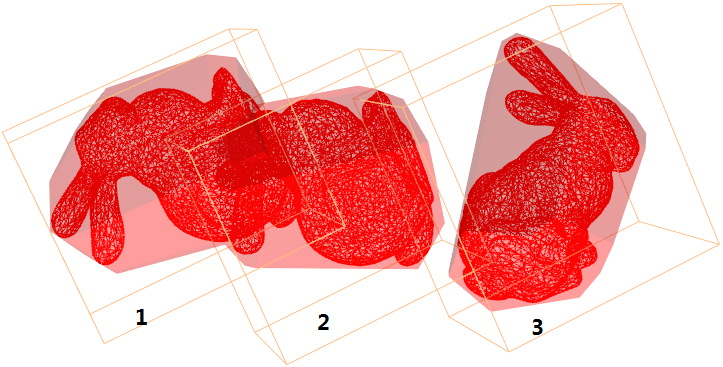
\includegraphics[width=4.5in]{bunny-box-kcbp-collsion-detection-example.png}
\caption{~$k-$CBP~应用于碰撞检测示例}
\label{lbl:bunny-box-kcbp-collsion-detection-example}
\end{figure}


\section{实验结果}
\label{sec:exper-cd}

[TODO]


本文实验通过生成不同数量的模型(模型位置和旋转角度随机生成), 碰撞检测时首先判断包围盒是否相交, 然后判断凸包围多面体是否相交, 最后再判断实际模型是否相交.
凸包围多面体之间的碰撞检测时可采用文献~${[27]}$~中提到的方法,
本文案例中模型和凸包围多面体是否相交都采用了普通~AABB~树的方式进行判断,
从如表~\ref{tab:exp:box:kcbp:collsiondetection}~的实验结果可看出含有凸包多围体的模型之间的碰撞检测算法能显著提高整体应用的效率. 

\begin{table}[htbp]
\caption{$k$-CBP~和包围盒应用于碰撞检测结果对比}
\label{tab:exp:box:kcbp:collsiondetection}
\centering
 \begin{tabular}{lccccccl}
 \toprule[1.5pt]
  n& c(Box)(ms) & c($16$-CBP)(ms) &  t(Box)(ms) & t($16$-CBP)(ms) & r(Box)(\%) & r($k$-CBP)(\%) & n(Model) \\
  \midrule[1.0pt]
%  10 & 0.1 & 1.8 & 26.0  & 0.1 & 2 & 0 & 0\\
%  30 & 0.2 & 2.9 & 134.0  & 70.0 & 11 & 6 & 5\\
%  50 & 0.5 & 4.8 & 506.0  & 255.2 & 41 & 22 & 19 \\
%  70 & 0.4 & 4.8 & 901.1  & 492.5 & 77 & 42 & 34 \\
%  90 & 0.7 & 5.7 & 1324.0  & 734.7 & 110 & 63 & 46 \\
%  100 & 0.7 & 7.8 & 1481.0  & 870.7 & 127 & 73 & 55 \\
%  150 & 1.0 & 9.8 & 4153.1  & 2473.0 & 349 & 212 & 150 \\
%  200 & 1.6 & 12.8 & 8049.3 & 4430.9 & 685 & 394 & 281 \\
   10 & 0.1 & 1.8 &    26.0  & 0.1    & 0.00  & 100.00 & 0\\
   30 & 0.2 & 2.9 &   134.0  & 70.0   & 45.45 & 83.33 & 5\\
   50 & 0.5 & 4.8 &   506.0  & 255.2  & 46.34 & 86.36 & 19 \\
   70 & 0.4 & 4.8 &   901.1  & 492.5  & 44.16 & 80.95 & 34 \\
   90 & 0.7 & 5.7 &  1324.0  & 734.7  & 41.82 & 73.02 & 46 \\
  100 & 0.7 & 7.8 &  1481.0  & 870.7  & 43.31 & 75.34 & 55 \\
  150 & 1.0 & 9.8 &  4153.1  & 2473.0 & 42.98 & 70.75 & 150 \\
  200 & 1.6 & 12.8 & 8049.3  & 4430.9 & 41.02 & 71.32 & 281 \\
  \bottomrule[1.5pt]
 \end{tabular}
\end{table}

如表~\ref{tab:exp:box:kcbp:collsiondetection}~所示,
其中~n~表示场景中模型的数量, c(Box), c($16$-CBP)分别表示模型包围盒的构造时间和凸包围16面体的构造时间(单位ms), t(Box), t($16$-CBP)~分表表示用包围盒进行碰撞检测和利用凸包围16面体进行碰撞检测所耗费的时间,
其中~r(Box), r($16$-CBP)分别表示包围盒、16-CBP~的命中率(即用实际模型相交的数量除以包围体检测出来相交的数量), ~n(Model)模型实际相交的数量, 显然计算模型包围盒所耗费的时间要明显少于计算凸包围多面体的时间, 但由于凸包围多面体比包围盒紧致,
因而命中率比包围盒高, 能排除更多本不相交的模型进而节省碰撞检测总时间, 提高算法效率.
